\section{Cronograma}

\begin{figure}[!ht]
    \centering
    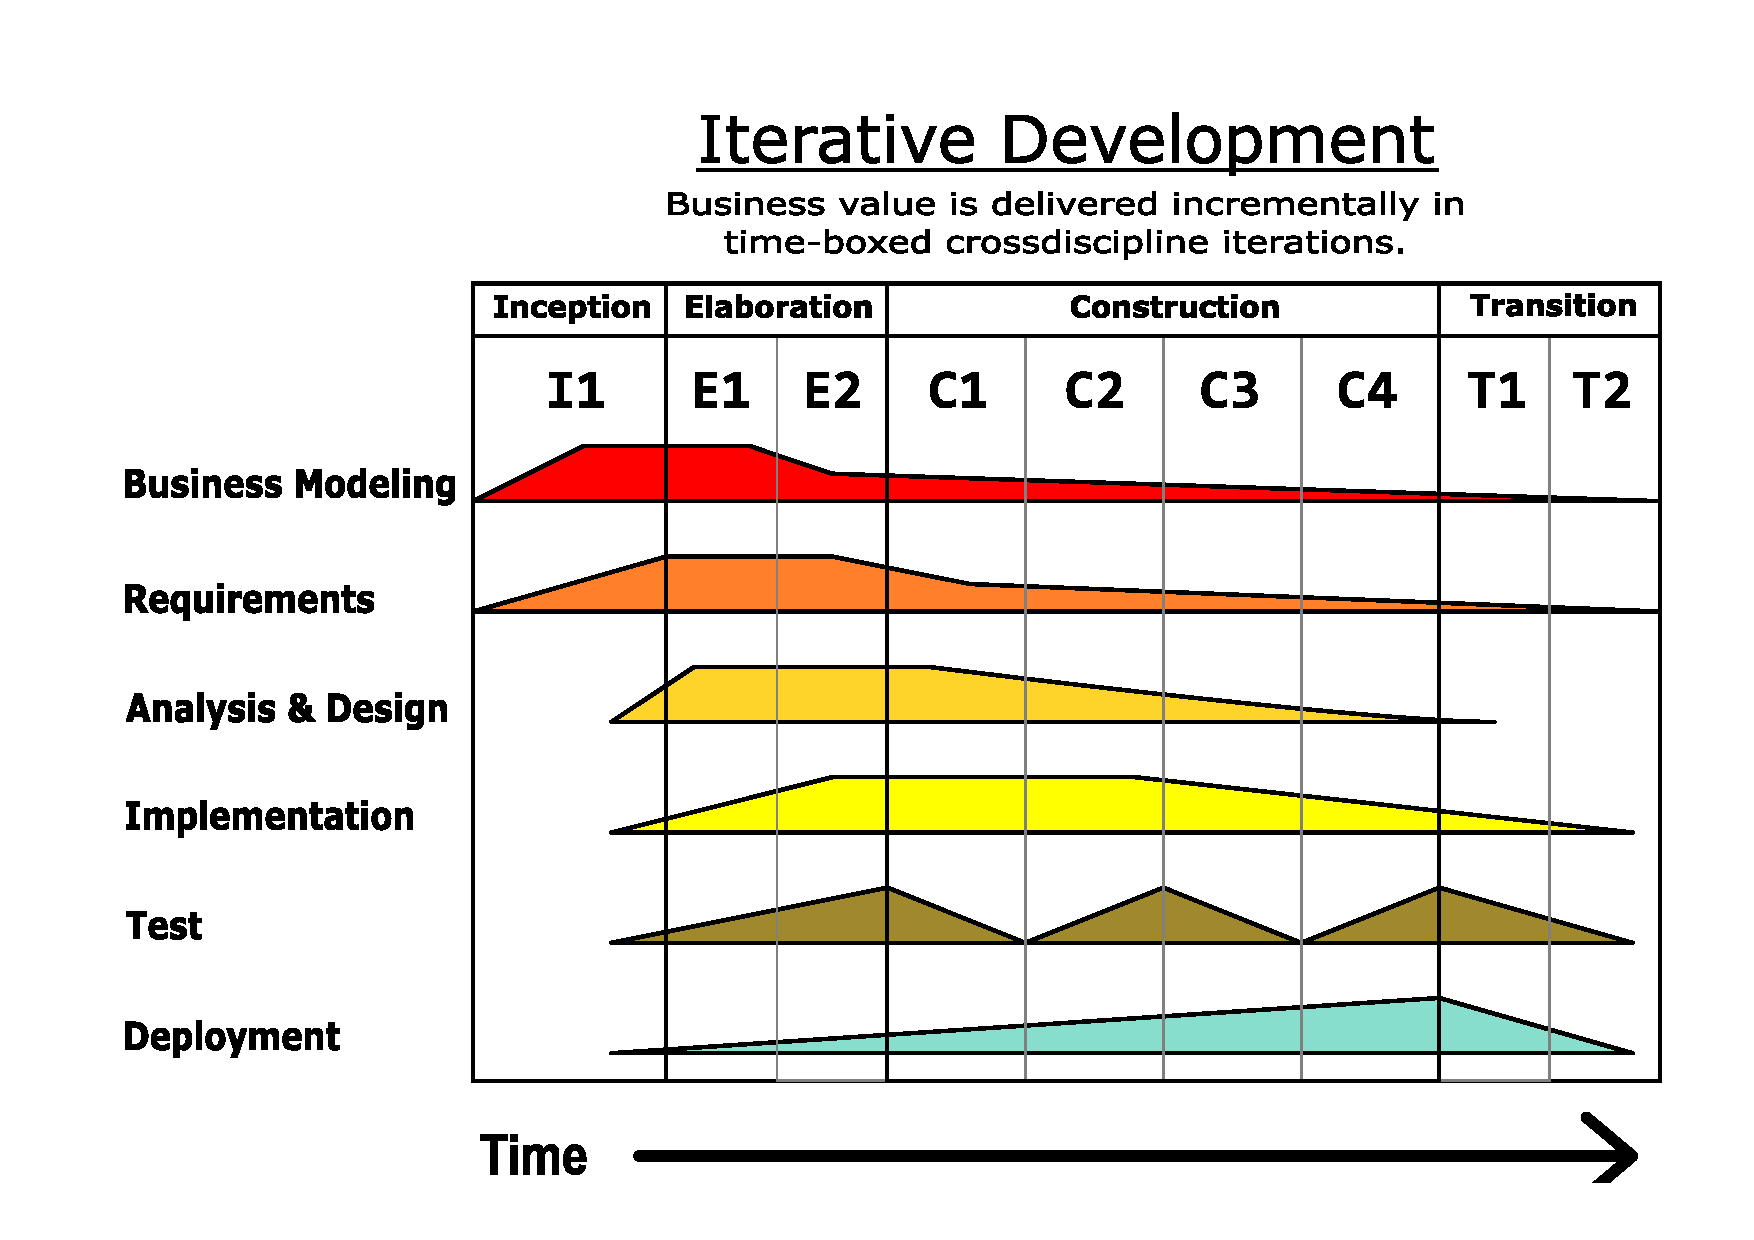
\includegraphics[width=0.7\textwidth]{assets/rupphases}
    \caption{Fases del Proceso Unificado y los esfuerzos de cada actividad en las mismas}
    \label{fig:rupphases}
\end{figure}

El cronograma de trabajo (figura \ref{fig:gantt}) estará fuertemente influenciado por las fases de la metodología \textit{RUP (Rational Unified Process)}, la cual cuenta con 4 fases y 6 actividades principales que se realizan de forma iterativa en cada una de estas fases. La figura \textit{\ref{fig:rupphases}} muestra cuánto de cada actividad se debe realizar en cada etapa y permite entender el cronograma presentado.

\begin{figure}
    
\begin{ganttchart}[
        vgrid,
        hgrid,
        x unit=\textwidth/33,
        bar label node/.append style={text width=2.5cm, align=right}
    ]{1}{25}
    % TITLE
    \gantttitle{Tunkunia - 25 Semanas}{25} \\
    \gantttitlelist{1,...,25}{1} \\

    % Tareas generales
    \ganttbar{Investigación}{1}{2} \\
    \ganttbar[name=mem0]{Redacción Memoria}{4}{7}
    \ganttbar[name=mem1]{Redacción Memoria}{16}{18}
    \ganttbar[name=mem2]{Redacción Memoria}{22}{25} \\
    \ganttlinkedmilestone{Presentación}{25} \\

    % Tareas del desarrollo en sí mismo
    \ganttgroup[name=rup]{Iteraciones RUP}{3}{18} \\
    \ganttbar[name=in]{Inception}{3}{4} \\
    \ganttlinkedbar{Elaboration}{5}{7} \\
    \ganttlinkedbar[name=const]{Construction}{8}{15} \\
    \ganttlinkedbar{Transition}{16}{17} \\
    \ganttlinkedbar[name=doc]{Documentación}{18}{18} \\

    % Aplicación y posteriores
    \ganttgroup[name=use]{Aplicación}{19}{22} \\
    \ganttbar[name=fork]{Fork del SIAI}{19}{19} \\
    \ganttlinkedbar{Integración}{20}{21} \\
    \ganttlinkedbar{Pruebas}{22}{22}

    % Milestones
    %\ganttlink{elem0}{in}
    \ganttlink{doc}{fork}
    %\ganttlink{const}{mem}
\end{ganttchart}
    \caption{Diagrama de Gantt del proyecto}
    \label{fig:gantt}
\end{figure}
Se debe notar que la redacción de la memoria se realizará de forma paralela al desarrollo del proyecto, al igual que el proceso de Investigación. Sin embargo, en el diagrama de Gantt se muestran las semanas en las que estas dos actividades tomarán prioridad.